% =====================================================================
%  Final-Year Research Project Report
%  Department of Computer Science, University of Jaffna
%  Compile with pdfLaTeX + BibTeX (Overleaf default settings work).
% =====================================================================
\documentclass[12pt,a4paper,oneside]{report}

% ---------- Encoding and fonts ----------
\usepackage[T1]{fontenc}
\usepackage[utf8]{inputenc}
\usepackage{lmodern}
\usepackage{microtype}

% ---------- Page layout ----------
\usepackage[a4paper,left=30mm,right=25mm,top=25mm,bottom=25mm]{geometry}
\usepackage{setspace}
\onehalfspacing
\setlength{\parskip}{4pt}

% ---------- Mathematics ----------
\usepackage{amsmath,amssymb}
\usepackage{bm}

% ---------- Tables ----------
\usepackage{booktabs}
\usepackage{tabularx}
\usepackage{multirow}
\usepackage{array}
\usepackage{longtable}
\newcolumntype{Y}{>{\raggedright\arraybackslash}X}
\newcolumntype{C}[1]{>{\centering\arraybackslash}p{#1}}

% ---------- Figures ----------
\usepackage{graphicx}
\usepackage{float}
\usepackage{caption}
\captionsetup{font=small,labelfont=bf}
\usepackage{subcaption}
\usepackage{tikz}
\usetikzlibrary{arrows.meta,positioning,shapes.geometric,fit,calc,backgrounds}
\usepackage{pgfplots}
\pgfplotsset{compat=1.17}

% ---------- Lists, colour, misc ----------
\usepackage{enumitem}
\setlist{itemsep=2pt,topsep=4pt}
\usepackage{xcolor}
\usepackage[nottoc]{tocbibind}
\usepackage{titlesec}
\titleformat{\chapter}[display]{\normalfont\Large\bfseries}{\chaptertitlename\ \thechapter}{10pt}{\LARGE}
\titlespacing*{\chapter}{0pt}{-10pt}{20pt}

% ---------- Citations and links ----------
\usepackage{cite}
\usepackage[hidelinks]{hyperref}
\usepackage[nameinlink,capitalise]{cleveref}

% ---------- Project-wide macros (edit here if details change) ----------
\newcommand{\reporttitle}{Lightweight Graph Neural Networks for QoS-Aware Delay Prediction in Software-Defined Networks}
\newcommand{\studentname}{K. Abaragithan}
\newcommand{\regno}{2021/SP/061}
\newcommand{\supervisor}{Dr. K. Thabotharan}
\newcommand{\department}{Department of Computer Science}
\newcommand{\university}{University of Jaffna}
\newcommand{\submissiondate}{December 2026}

% Short names used throughout the text
\newcommand{\rnf}{RouteNet-Fermi}
\newcommand{\qlf}{Queue-Link Fusion}

\begin{document}

% ---------------------------------------------------------------------
\pagenumbering{roman}
\begin{titlepage}
\centering
\vspace*{10mm}

{\large \university\par}
\vspace{2mm}
{\large \department\par}

\vspace{25mm}

{\LARGE\bfseries \reporttitle\par}

\vspace{20mm}

{\large A research project report submitted in partial fulfilment of the requirements for the degree of\par}
\vspace{3mm}
{\large\itshape Bachelor of Science Honours in Computer Science\par}

\vspace{25mm}

\begin{tabular}{rl}
\textbf{Student:} & \studentname \\[2mm]
\textbf{Registration Number:} & \regno \\[2mm]
\textbf{Supervisor:} & \supervisor \\[2mm]
\textbf{Course:} & CSC406S6 / CSC406M6 Research Project \\
\end{tabular}

\vfill

{\large \submissiondate\par}
\end{titlepage}

\chapter*{Declaration}
\addcontentsline{toc}{chapter}{Declaration}

I declare that this report describes work carried out by me under the supervision of \supervisor{}, and that it has not been submitted, in whole or in part, for any other degree or qualification. Where the work of others has been used, including published papers, datasets and source code, it is acknowledged in the text and listed in the references.

\vspace{20mm}

\noindent
\begin{tabular}{@{}p{70mm}p{70mm}@{}}
\rule{60mm}{0.4pt} & \rule{60mm}{0.4pt} \\
\studentname{} (\regno) & Date \\[18mm]
\rule{60mm}{0.4pt} & \rule{60mm}{0.4pt} \\
\supervisor{} (Supervisor) & Date \\
\end{tabular}

% NOTE TO AUTHOR: personalise this page before submission.
\chapter*{Acknowledgements}
\addcontentsline{toc}{chapter}{Acknowledgements}

I thank my supervisor, \supervisor{}, for guidance throughout this project, and the staff of the \department{}, \university{}, for their support.

The experiments in this report build on the RouteNet-Fermi model and the all-mixed dataset published by the Barcelona Neural Networking Center at Universitat Polit\`ecnica de Catalunya under the Apache License 2.0. I am grateful to the authors for making them openly available.

\chapter*{Abstract}
\addcontentsline{toc}{chapter}{Abstract}

Software-defined networking (SDN) controllers can use a network model to estimate per-flow delay before changing routes. Graph neural network (GNN) models such as RouteNet-Fermi are accurate but costly, and depend on how well their training data cover the networks met in operation. This project investigates whether a smaller GNN, trained with help from a larger one, can give usable delay estimates at lower cost. Training RouteNet-Fermi on 10- to 170-node instead of only 10-node topologies lowered the mean absolute percentage error (MAPE) on 478 unseen 200- to 300-node scenarios from 8.40\% to 5.37\%. A lightweight student, Queue-Link Fusion, merges each link with its queues, cutting message passing from 24 to 8 stages and parameters from 27,025 to 4,505. Its forward pass was 4.4 to 7.9 times faster on a CPU, but end to end the saving was only about 8\%, because building the input graph took about 90\% of the time. The student's error was about twice the teacher's. A first distillation run lowered it from 11.92\% to 9.83\%, but a controlled re-test with three paired seeds, identical initial weights and a relative distillation loss showed no consistent benefit: the distilled student was better in two pairs and worse in one on validation, and \pending{test result pending}. The student's training error (7.1\%) already exceeded the teacher's validation error (4.7\%), so its limit is capacity rather than guidance. In a six-switch Mininet emulation with a Ryu controller, all three frozen models ranked three candidate paths in the measured order of delay, and the chosen path had 8.8\% lower delay than the hop-count default. An Abilene emulation failed because its traffic lay far outside the training range. Topology diversity improved accuracy, but compression cost more than diversity recovered, and graph construction, not the model, dominated the cost.

\vspace{4mm}
\noindent\textbf{Keywords:} software-defined networking, graph neural networks, network modelling, knowledge distillation, Mininet, out-of-distribution generalisation


\tableofcontents
\listoffigures
\listoftables
\chapter*{List of Abbreviations}
\addcontentsline{toc}{chapter}{List of Abbreviations}

{\small
\begin{tabular}{@{}p{14mm}p{56mm}p{13mm}p{56mm}@{}}
APE  & Absolute Percentage Error      & MP   & Message Passing \\
CBR  & Constant Bit Rate              & MSE  & Mean Squared Error \\
DRL  & Deep Reinforcement Learning    & OOD  & Out-of-Distribution \\
FIFO & First In, First Out            & QoS  & Quality of Service \\
GNN  & Graph Neural Network           & SDN  & Software-Defined Networking \\
GRU  & Gated Recurrent Unit           & SP   & Strict Priority \\
KD   & Knowledge Distillation         & ToS  & Type of Service \\
MAPE & Mean Absolute Percentage Error & UDP  & User Datagram Protocol \\
MLP  & Multi-Layer Perceptron         & WFQ  & Weighted Fair Queueing \\
\end{tabular}
}


% ---------------------------------------------------------------------
\clearpage
\pagenumbering{arabic}
\chapter{Introduction}
\label{ch:intro}

\section{Background and Motivation}
\label{sec:background}

Software-defined networking (SDN) separates the control plane of a network from its data plane and places routing and configuration decisions in a logically centralised controller \cite{kreutz2015sdn,mckeown2008openflow}. Because the controller has a global view of the topology and can reprogram forwarding behaviour, it is a natural place to apply quality-of-service (QoS) policies: choosing paths that keep end-to-end delay low, spreading load to avoid congestion, or assigning traffic classes to queues with suitable scheduling. To make such decisions well, the controller needs some way of predicting how a candidate configuration will perform before it is deployed. This is the role of a \emph{network model}.

Two classical kinds of network model are in common use. Analytical models based on queueing theory \cite{kleinrock1975queueing} are fast, but they rest on assumptions, such as Poisson arrivals and independence between queues, that real traffic and multi-hop paths often violate. Packet-level simulators such as OMNeT++ \cite{varga2001omnet} and ns-3 \cite{riley2010ns3} are accurate, but simulating a large network under realistic load can take minutes to hours, which rules them out for decisions that have to be made while the network is running. Knowledge-defined networking \cite{mestres2017kdn} proposed closing this gap with models learned from data.

Graph neural networks (GNNs) \cite{scarselli2009gnn,gilmer2017mpnn,battaglia2018relational} have turned out to suit this task well, because a network is itself a graph and the quantities of interest (per-flow delay, jitter and loss) emerge from interactions between flows, links and queues. RouteNet \cite{rusek2020routenet} showed that a GNN which passes messages between paths and links can predict per-path delay on topologies it was not trained on. RouteNet-Fermi \cite{ferriolgalmes2023routenetfermi} extended this design with explicit queue entities, multiple traffic models and four scheduling policies, and reported accuracy close to packet-level simulation at a small fraction of its cost.

These models still leave two practical problems, and both motivate this project.

The first problem is \emph{computational cost on small controllers}. RouteNet-Fermi performs eight iterations of three message-passing stages, each driven by a recurrent unit, over a graph that for a few hundred nodes can contain tens of thousands of flows. On the CPU-only machine used in this project, a single forward pass of RouteNet-Fermi on one validation sample took about 178~ms (\cref{sec:efficiency}). That is acceptable for occasional what-if analysis in a data centre, but it is less attractive for controllers running on edge hardware that must evaluate many candidate configurations quickly.

The second problem is \emph{generalisation to larger networks}. A learned model is only reliable on inputs that resemble its training data, and operational networks are often larger than the ones that can be simulated cheaply to produce training data. A model trained only on small topologies may degrade on large ones, and it is not obvious in advance by how much.

Knowledge distillation (KD) \cite{hinton2015distilling,gou2021kdsurvey} offers one way to address both problems together. A large, accurate \emph{teacher} model is trained first, ideally on data that cover a wide range of conditions, and a small \emph{student} model is then trained to match both the ground truth and the teacher's outputs. KD has been studied extensively for GNNs in node classification and recommendation \cite{yang2020lsp,zhang2022glnn,chen2021gnnsd,yang2023ltd,huo2023t2gnn,chen2025lightgnn}, but much less for regression models that predict network performance, where the target is a continuous delay value and the evaluation that matters is accuracy on unseen, larger topologies.

\section{Research Aim and Objectives}
\label{sec:objectives}

The aim of this project is to determine whether a lightweight GNN, trained with knowledge distillation from a topology-diverse RouteNet-Fermi teacher, can predict per-flow delay in SDN-like networks at a substantially lower computational cost, and to measure how much accuracy it gives up on topologies larger than any used in training.

The project has three objectives:

\begin{enumerate}[label=\textbf{O\arabic*.}, leftmargin=*]
  \item To reproduce RouteNet-Fermi delay prediction on the all-mixed dataset and quantify how its accuracy on held-out 200- to 300-node topologies changes when the training data are extended from 10-node topologies only to topologies of 10 to 170 nodes.
  \item To design and implement a lightweight student GNN that reduces the parameter count and the number of message-passing stages of RouteNet-Fermi while keeping its physically motivated delay readout.
  \item To train the student with and without knowledge distillation from the teacher, and to evaluate the trade-off between out-of-distribution accuracy, model size and inference latency against the full-size models.
\end{enumerate}

\section{Scope and Changes from the Research Proposal}
\label{sec:scope}

The original proposal \cite{proposal2025} described a broader programme: an SDN testbed built with Mininet and the RYU controller, compression by pruning, quantisation and distillation, and comparison against shortest-path and deep reinforcement learning (DRL) routing. During the project the work was narrowed, for two reasons. First, building a reliable learned model of network delay is a precondition for any routing scheme that relies on one, and on the available CPU-only hardware the study of out-of-distribution accuracy alone needed training runs of up to 13 hours and test-set evaluations of about two and a half hours per model. Second, the public all-mixed dataset provided simulator-generated ground truth at a scale (more than 12,000 labelled network scenarios) that could not have been produced with a Mininet testbed in the time available.

As a result, this report covers delay prediction only. Jitter and packet loss, pruning and quantisation, deployment on an SDN controller, and routing-decision experiments were not carried out, and no results are claimed for them. They are discussed as future work in \cref{sec:future}.

\section{Organisation of the Report}

\Cref{ch:related} reviews related work on network performance modelling, learning-based routing and knowledge distillation for GNNs, and identifies the gap this project addresses. \Cref{ch:method} describes the teacher model, the proposed student architecture and the distillation procedure. \Cref{ch:setup} sets out the dataset, data splits, implementation and evaluation protocol. \Cref{ch:results} presents and discusses the results. \Cref{ch:conclusion} summarises the findings and contributions and outlines future work. The appendices give per-epoch training records, a reproducibility guide and a preliminary experiment with the original RouteNet.

\chapter{Related Work}
\label{ch:related}

The literature relevant to this project falls into four groups: classical approaches to estimating network performance, learned network models (with GNN-based models as the main line), learning-based routing in SDN, and model compression with an emphasis on knowledge distillation for GNNs. The chapter closes with a comparison across these groups and a statement of the research gap.

\section{Analytical and Simulation-Based Performance Models}
\label{sec:rw-classic}

Queueing theory gives closed-form or numerically cheap estimates of delay and loss for individual queues and, under product-form assumptions, for networks of queues \cite{kleinrock1975queueing}. Its strength is speed and interpretability. Its weakness is that the assumptions needed for tractability (Markovian arrivals, independence between queues, simple scheduling) are routinely broken in practice. Bursty or autocorrelated traffic, priority and weighted-fair scheduling, and correlation between hops along a path all push measured delay away from the analytical estimate. Ferriol-Galm\'es et~al.\ \cite{ferriolgalmes2023routenetfermi} include a queueing-theory baseline in their evaluation and find it considerably less accurate than their learned model once traffic departs from the Poisson assumption.

Discrete-event packet simulators, such as OMNeT++ \cite{varga2001omnet} and ns-3 \cite{riley2010ns3}, model every packet and so capture these effects faithfully. The price is run time, which grows with the number of packets and therefore with network size and load. Simulators are the usual source of ground truth for training learned models, including the dataset used in this project, but they are too slow to sit inside a controller's decision loop. Kim et~al.\ \cite{kim2022drlsdn} make a similar observation from the routing side: they train a DRL agent against an offline M/M/1/K queueing model precisely because interacting with a live network or a full simulator during training would be too slow and too disruptive.

The two families therefore occupy opposite ends of a speed--accuracy spectrum, and the motivation for learned models is to occupy the middle of it.

\section{Learned Network Models}
\label{sec:rw-learned}

\subsection{Non-graph models}

Early learned network models treated the network as a fixed-size input vector. The knowledge-defined networking proposal \cite{mestres2017kdn} trained a multi-layer perceptron to map a traffic matrix to delay for one specific topology. Such models do not transfer to a different topology, because the input layout is tied to the topology on which they were trained. Later systems kept accuracy but changed the abstraction. MimicNet \cite{zhang2021mimicnet} learns per-cluster models of a data-centre network and composes them to estimate the behaviour of a much larger fabric, and DeepQueueNet \cite{yang2022deepqueuenet} learns packet-level device models that are assembled into a network-wide simulation. Both scale better than packet simulation, but both are designed around data-centre structure or around replaying packet traces, which is a different setting from per-flow delay prediction for arbitrary wide-area topologies.

\subsection{Graph neural network models}

GNNs \cite{scarselli2009gnn,gilmer2017mpnn,battaglia2018relational} compute a hidden state for every entity in a graph by repeatedly exchanging messages with neighbouring entities. Because the same learned functions are applied to every node and edge, a trained GNN can be run on graphs of a different size and shape from those it saw in training, which is the property that network modelling needs.

RouteNet \cite{rusek2020routenet} introduced a GNN tailored to networks. It represents links and paths as two sets of entities and alternates between updating each path from the links it traverses (using a recurrent unit over the ordered link sequence) and updating each link from the paths that cross it. Trained on simulated data, RouteNet predicted per-path delay and jitter on topologies outside its training set and was used inside an optimisation loop to choose routings that meet delay targets. Its main limitation was that it assumed a single first-in, first-out queue per link and Poisson-like traffic.

RouteNet-Erlang \cite{ferriolgalmes2022routeneterlang} and then RouteNet-Fermi \cite{ferriolgalmes2023routenetfermi} removed these limitations. RouteNet-Fermi adds queues as a third entity type, so that a link can host several queues with different priorities and weights, and supports four scheduling policies (FIFO, strict priority, WFQ and DRR) and several traffic models, including on--off and autoregressive sources. Rather than outputting delay directly, it predicts per-hop queue occupancy and converts it to delay using the link capacity, which makes the output scale correctly when link speeds change. The authors report that this design generalises to networks larger than those used for training. RouteNet-Fermi is the teacher architecture in this project and is described in detail in \cref{sec:teacher}.

A shared feature of this line of work is that model size and computational cost are not the main concern. RouteNet-Fermi uses three gated recurrent unit (GRU) cells \cite{cho2014gru}, 32-dimensional states and eight message-passing iterations. Jiang et~al.\ \cite{jiang2024gnnrouting} identify scalability, inference latency and memory use as open problems for GNNs in routing optimisation, and the RouteNet papers themselves evaluate accuracy and generalisation rather than deployment cost on constrained hardware.

\section{Learning-Based Routing in SDN}
\label{sec:rw-routing}

A related body of work uses learning to make routing decisions directly. Kim et~al.\ \cite{kim2022drlsdn} train a DRL agent to set link weights so as to reduce end-to-end delay and loss in SDN. Song et~al.\ \cite{song2024qosdrl} use deep deterministic policy gradient with a reward that combines delay, bandwidth, jitter and loss. Almasan et~al.\ \cite{almasan2022drlgnn} show that a DRL agent built on a GNN generalises across topologies far better than one built on a fully connected network, because the GNN does not tie its input to a fixed topology. He et~al.\ \cite{he2024causality} add causality detection to a GNN-based DRL agent to make it more stable under noisy conditions, and Ampratwum and Nayak \cite{ampratwum2025wdm} combine DRL and GNNs for restoration in optical networks.

These works matter to this project in two ways. First, several of them depend, during training or at decision time, on a model that estimates the consequence of an action; a fast and accurate delay model is therefore a building block for this kind of routing. Second, their evaluations generally measure routing quality rather than inference cost, and those that use GNNs inherit the computational load of the underlying GNN. Neither line of work, as reviewed here, studies how small the network model can be made before its predictions become unreliable.

\section{Model Compression and Knowledge Distillation}
\label{sec:rw-kd}

\subsection{General compression techniques}

Compression methods reduce the cost of running a trained network. Pruning removes weights or structures that contribute little \cite{han2016deepcompression}, and quantisation stores and computes with low-precision integers in place of 32-bit floats \cite{jacob2018quantization}. Both start from a trained architecture and make it cheaper while keeping its structure. Knowledge distillation \cite{hinton2015distilling} instead trains a separate, smaller model. In its original form the student is trained on a weighted sum of the usual loss against ground-truth labels and a loss that matches the teacher's softened output distribution; later variants also match intermediate representations \cite{romero2015fitnets}. A survey by Gou et~al.\ \cite{gou2021kdsurvey} classifies the many variants by what knowledge is transferred (responses, features or relations) and how (offline, online or self-distillation). Distillation is attractive when the desired student differs structurally from the teacher, which is the case in this project.

\subsection{Distillation for graph neural networks}

Applying distillation to GNNs raises the question of what graph-specific knowledge should be transferred. Yang et~al.\ \cite{yang2020lsp} propose a local-structure-preserving module that makes the student reproduce the teacher's view of how each node relates to its neighbours, not only its final outputs. Zhang et~al.\ \cite{zhang2022glnn} distil a GNN into a plain MLP that uses no graph structure at inference time; the resulting student is much faster but can only rely on the features of each node, which suits node classification on a fixed graph. Chen et~al.\ \cite{chen2021gnnsd} remove the separate teacher altogether and propose self-distillation, in which a GNN regularises its own deeper layers using a measure of how much each node's embedding differs from its neighbourhood. Yang et~al.\ \cite{yang2023ltd} learn distillation temperatures for individual nodes jointly with the student, rather than using one global temperature. Huo et~al.\ \cite{huo2023t2gnn} use two teachers, one specialised in node features and one in graph structure, to train a student that copes with graphs whose features and edges are partly missing. LightGNN \cite{chen2025lightgnn} combines pruning with hierarchical distillation to compress GNN-based recommender models.

Two features of this work are worth noting for the present project. First, almost all of it concerns classification or ranking: the teacher's output is a probability distribution or a score, and temperature-softened outputs carry ``dark knowledge'' about relative class similarity. Per-flow delay is a continuous regression target with no such distribution, so the classical soft-label loss does not apply directly and a regression loss on the teacher's predictions has to be used instead. Second, the student architectures studied are usually smaller copies of the teacher, or MLPs that drop the graph entirely. A network model cannot drop the graph, because the delay of a flow depends on what other flows share its links and queues, so a student for this task has to remain a GNN while still being cheaper.

\section{Synthesis and Research Gap}
\label{sec:gap}

\Cref{tab:rw-compare} compares representative work along the dimensions that matter for this project.

\begin{table}[ht]
\centering
\small
\caption{Comparison of representative related work against the requirements of this project.}
\label{tab:rw-compare}
\begin{tabularx}{\textwidth}{@{}l Y C{19mm} C{19mm} C{17mm}@{}}
\toprule
\textbf{Approach} & \textbf{Representative work} & \textbf{Per-flow QoS} & \textbf{Unseen topologies} & \textbf{Low cost} \\
\midrule
Queueing theory      & \cite{kleinrock1975queueing}                       & Approx. & Yes & Yes \\
Packet simulation    & \cite{varga2001omnet,riley2010ns3}                 & Yes     & Yes & No  \\
Non-graph learned    & \cite{mestres2017kdn,zhang2021mimicnet,yang2022deepqueuenet} & Partly & Limited & Partly \\
GNN network models   & \cite{rusek2020routenet,ferriolgalmes2022routeneterlang,ferriolgalmes2023routenetfermi} & Yes & Yes & Not studied \\
DRL / DRL+GNN routing & \cite{kim2022drlsdn,song2024qosdrl,almasan2022drlgnn,he2024causality} & Decision, not estimate & Partly & Not studied \\
GNN distillation     & \cite{yang2020lsp,zhang2022glnn,chen2021gnnsd,yang2023ltd,huo2023t2gnn} & Not addressed & n/a & Yes \\
\bottomrule
\end{tabularx}
\end{table}

The comparison shows a clear gap. GNN network models such as RouteNet-Fermi provide accurate per-flow estimates that transfer across topologies, but their computational cost on constrained hardware has not been the subject of study. GNN distillation methods reduce cost, but they have been developed and evaluated for classification and recommendation, with students that are either smaller copies of the teacher or graph-free MLPs. No reviewed work has examined whether a structurally simpler GNN student, distilled from a network-modelling teacher, can keep useful delay accuracy, nor how such a student behaves on topologies larger than those seen in training. A related point, which emerges from the experiments in \cref{ch:results}, is that the choice of training topologies for the teacher itself has a large effect on this out-of-distribution accuracy.

This project addresses that gap by (i) measuring the effect of topology diversity on RouteNet-Fermi's accuracy on larger, unseen topologies, (ii) proposing a student architecture that merges queues into links to shorten message passing, and (iii) evaluating the student with and without distillation on the same held-out topologies.

\chapter{Methodology}
\label{ch:method}

This chapter describes the approach taken to meet the objectives in \cref{sec:objectives}. It first gives the overall workflow, then formulates the prediction problem, describes the teacher (RouteNet-Fermi) and the proposed student (Queue-Link Fusion), and finally sets out how the student is trained with knowledge distillation.

\section{Overall Workflow}
\label{sec:workflow}

\Cref{fig:workflow} summarises the workflow. The same data pipeline turns each simulated network scenario into a graph, and four models are trained from it. The \emph{baseline} is RouteNet-Fermi trained on the dataset's original training split, which contains only 10-node topologies. The \emph{teacher} has the same architecture but is trained on a re-split of the data that includes topologies of 10 to 170 nodes. The \emph{student} is trained twice on the same re-split: once on the ground truth alone (\emph{student-scratch}) and once with distillation from the frozen teacher (\emph{student-KD}). All four models are then evaluated on one held-out test set of 200- to 300-node topologies, and their size and inference latency are measured.

\begin{figure}[ht]
\centering
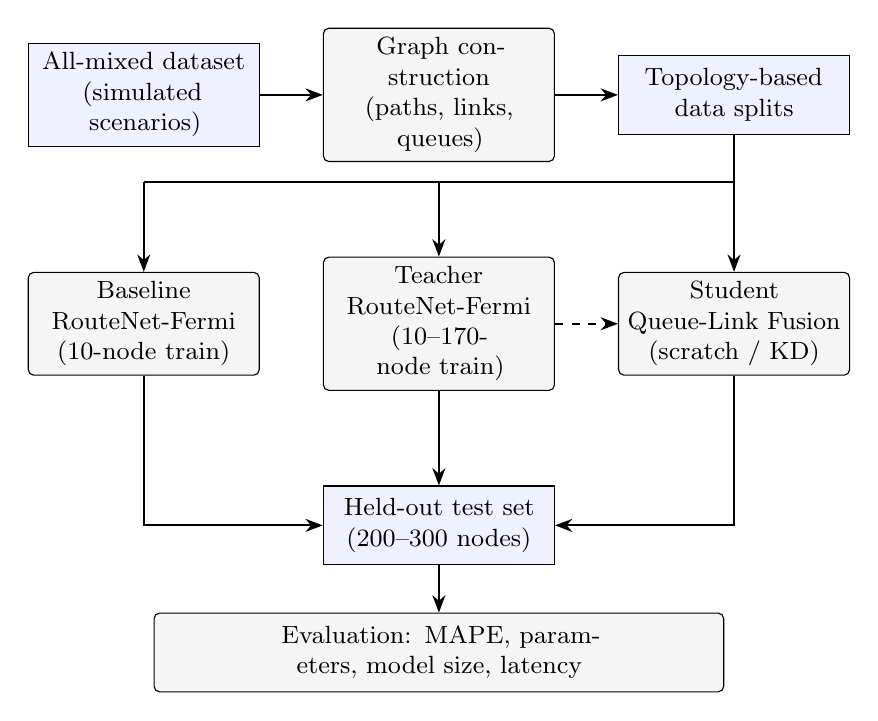
\begin{tikzpicture}[
  node distance=6mm and 8mm,
  box/.style={draw, rounded corners=2pt, align=center, font=\small, minimum height=10mm, text width=27mm, fill=gray!8},
  data/.style={draw, align=center, font=\small, minimum height=10mm, text width=27mm, fill=blue!6},
  arr/.style={-{Stealth[length=2.2mm]}, thick}
]
\node[data] (raw) {All-mixed dataset\\(simulated scenarios)};
\node[box, right=of raw] (hg) {Graph construction\\(paths, links, queues)};
\node[data, right=of hg] (split) {Topology-based\\data splits};

\node[box, below=12mm of hg] (teach) {Teacher\\RouteNet-Fermi\\(10--170-node train)};
\node[box, left=8mm of teach] (base) {Baseline\\RouteNet-Fermi\\(10-node train)};
\node[box, right=8mm of teach] (stud) {Student\\Queue-Link Fusion\\(scratch / KD)};

\node[data, below=12mm of teach] (test) {Held-out test set\\(200--300 nodes)};
\node[box, below=6mm of test, text width=70mm] (eval) {Evaluation: MAPE, parameters, model size, latency};

\draw[arr] (raw) -- (hg);
\draw[arr] (hg) -- (split);
\coordinate (bus) at ($(split.south)+(0,-6mm)$);
\draw[thick] (split.south) -- (bus);
\draw[thick] (base.north |- bus) -- (stud.north |- bus);
\draw[arr] (base.north |- bus) -- (base.north);
\draw[arr] (teach.north |- bus) -- (teach.north);
\draw[arr] (stud.north |- bus) -- (stud.north);
\draw[arr, dashed] (teach) -- (stud);
\draw[arr] (base) |- (test);
\draw[arr] (teach) -- (test);
\draw[arr] (stud) |- (test);
\draw[arr] (test) -- (eval);
\end{tikzpicture}
\caption{Overall workflow of the project. The dashed arrow shows the teacher's predictions being used as an additional training signal for the student.}
\label{fig:workflow}
\end{figure}

\section{Problem Formulation}
\label{sec:problem}

A network scenario consists of a topology, a routing configuration and a traffic matrix. The topology has a set of directed links $\mathcal{L}$; each link $l$ has a capacity $c_l$ and inherits a scheduling policy $\pi_l \in \{\text{WFQ}, \text{SP}, \text{DRR}, \text{FIFO}\}$ from its source node. Each link has a set of output queues $\mathcal{Q}(l)$, with at most three queues per link. Queue $q$ has a buffer size $b_q$, a priority index $r_q$ and, for weighted policies, a normalised weight $w_q$.

Traffic is described by a set of flows $\mathcal{P}$, each following a fixed path. A path $p$ is an ordered sequence of links $(l_{p,1}, \dots, l_{p,|p|})$ and, at each hop $k$, uses the queue $q_{p,k}$ that its type-of-service (ToS) class maps to on that link. Each flow has a mean bit rate $\lambda_p$, a packet generation rate $n_p$, a traffic model $m_p$ (one of seven, encoded one-hot) and up to eight parameters of its time distribution $\bm{\theta}_p$.

The task is to predict, for every flow $p$ in a scenario, its mean end-to-end delay $y_p$ as measured by the packet-level simulator that generated the dataset. A model $f$ receives the whole scenario and outputs $\hat{y}_p$ for all flows at once. Accuracy is measured with the mean absolute percentage error,
\begin{equation}
\mathrm{MAPE} = \frac{100}{|\mathcal{P}|} \sum_{p \in \mathcal{P}} \frac{|y_p - \hat{y}_p|}{|y_p|},
\label{eq:mape}
\end{equation}
which is also the training loss for the baseline, the teacher and the scratch student. A relative error is used because delays in the dataset span more than two orders of magnitude (\cref{sec:datasets}), so an absolute error would be dominated by the slowest flows.

Two derived quantities are computed from the inputs before any learning takes place. The offered load of a link is
\begin{equation}
\rho_l = \frac{1}{c_l} \sum_{p \,:\, l \in p} \lambda_p ,
\label{eq:load}
\end{equation}
and the mean packet size of a flow is $s_p = \lambda_p / n_p$.

\section{Graph Representation}
\label{sec:graph}

Each scenario is converted into a graph whose nodes are of three types: \emph{paths}, \emph{links} and \emph{queues}. A path is connected to every link and every queue it traverses; a queue is connected to the link it belongs to. This representation follows RouteNet-Fermi \cite{ferriolgalmes2023routenetfermi} and is built by the data pipeline distributed with its reference implementation, which reads the simulator output through the dataset's API and produces, for each scenario, the feature tensors and index tensors needed for message passing (for example, which links and queues each path visits, in order).

The graphs are large. One scenario from the dataset's original test split, used during development to inspect the pipeline, contained 852 links, 2,124 queues and 57,360 flows, and therefore 57,360 delay labels. Every training step in this project processes one such scenario; there is no batching across scenarios.

\section{Teacher Model: RouteNet-Fermi}
\label{sec:teacher}

The teacher is RouteNet-Fermi \cite{ferriolgalmes2023routenetfermi}, used without architectural changes. It keeps a hidden state $\mathbf{h}_p$, $\mathbf{h}_l$ and $\mathbf{h}_q$ of dimension 32 for every path, link and queue.

\paragraph{Initial states.}
Each state is initialised by a two-layer MLP with ReLU activations applied to the entity's features, where $z(\cdot)$ denotes z-score normalisation with fixed dataset statistics:
\begin{align}
\mathbf{h}_p^{(0)} &= \mathrm{MLP}_p\big([\,z(\lambda_p),\, z(n_p),\, \mathrm{onehot}(m_p),\, z(\bm{\theta}_p)\,]\big) && \text{(17 inputs)}\\
\mathbf{h}_l^{(0)} &= \mathrm{MLP}_l\big([\,\rho_l,\, \mathrm{onehot}(\pi_l)\,]\big) && \text{(5 inputs)}\\
\mathbf{h}_q^{(0)} &= \mathrm{MLP}_q\big([\,z(b_q),\, \mathrm{onehot}(r_q),\, w_q\,]\big) && \text{(5 inputs)}
\end{align}

\paragraph{Message passing.}
The model then runs $T = 8$ iterations, each consisting of three stages.
\begin{enumerate}
  \item \emph{Links and queues to paths.} A GRU \cite{cho2014gru} reads, hop by hop, the concatenated states of the queue and link used at each hop, starting from the current path state:
  \begin{equation}
  \mathbf{s}_p^{(k)} = \mathrm{GRU}_p\big(\,[\mathbf{h}_{q_{p,k}} \,\|\, \mathbf{h}_{l_{p,k}}],\ \mathbf{s}_p^{(k-1)}\big), \qquad \mathbf{s}_p^{(0)} = \mathbf{h}_p,
  \end{equation}
  and the new path state is $\mathbf{h}_p \leftarrow \mathbf{s}_p^{(|p|)}$. The intermediate states $\mathbf{s}_p^{(k)}$ are kept.
  \item \emph{Paths to queues.} Each queue sums the states of the paths that use it, taken at the point where each path arrives at the queue, and updates its state with a second GRU cell:
  \begin{equation}
  \mathbf{h}_q \leftarrow \mathrm{GRU}_q\Big(\sum_{(p,k)\,:\,q_{p,k}=q} \mathbf{s}_p^{(k-1)},\ \mathbf{h}_q\Big).
  \end{equation}
  \item \emph{Queues to links.} Each link runs a third GRU over the states of its queues, starting from its own state, and keeps the final output as its new state.
\end{enumerate}

\paragraph{Readout.}
After the last iteration, an MLP (32--16--16--1) maps each per-hop path state to a value $o_{p,k}$ interpreted as the queue occupancy seen by flow $p$ at hop $k$. Delay is then computed from the physics of a store-and-forward network rather than predicted directly:
\begin{equation}
\hat{y}_p = \underbrace{\sum_{k=1}^{|p|} \frac{o_{p,k}}{c_{l_{p,k}}}}_{\text{queueing delay}} \;+\; \underbrace{s_p \sum_{k=1}^{|p|} \frac{1}{c_{l_{p,k}}}}_{\text{transmission delay}} .
\label{eq:readout}
\end{equation}
Dividing by link capacity means that the network only has to learn occupancy, which is less sensitive to the absolute link speed than delay itself. This is one of the reasons RouteNet-Fermi is reported to generalise to networks with link capacities outside the training range \cite{ferriolgalmes2023routenetfermi}.

In total the teacher has 27,025 trainable parameters, and each forward pass performs $8 \times 3 = 24$ message-passing stages.

\section{Proposed Student Model: Queue-Link Fusion}
\label{sec:student}

The student is designed to cut the cost of message passing while keeping the parts of RouteNet-Fermi that are most closely tied to how delay arises: the per-hop recurrent reading of each path and the capacity-based readout of \cref{eq:readout}.

\subsection{Design idea}

In a real router, the queues of a link are not independent objects; they are buffers on that link's output port, and their combined behaviour determines how long a packet waits before transmission on that link. The student exploits this by merging each link and its queues into a single \emph{interface} entity before message passing begins. The tripartite path--link--queue graph of the teacher becomes a bipartite path--interface graph (\cref{fig:graphs}). This removes the queue states, the queue GRU, the paths-to-queues stage and the queues-to-links stage.

\begin{figure}[ht]
\centering
\begin{subfigure}[b]{0.48\textwidth}
\centering
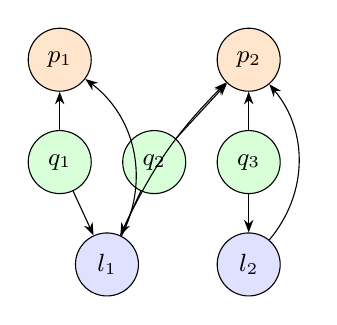
\begin{tikzpicture}[
  ent/.style={circle, draw, minimum size=8mm, font=\small, inner sep=0pt},
  every edge/.style={draw, -{Stealth[length=1.6mm]}, thin}
]
\node[ent, fill=orange!20] (p1) at (0,2.2) {$p_1$};
\node[ent, fill=orange!20] (p2) at (2.4,2.2) {$p_2$};
\node[ent, fill=green!15] (q1) at (0,0.9) {$q_1$};
\node[ent, fill=green!15] (q2) at (1.2,0.9) {$q_2$};
\node[ent, fill=green!15] (q3) at (2.4,0.9) {$q_3$};
\node[ent, fill=blue!12] (l1) at (0.6,-0.4) {$l_1$};
\node[ent, fill=blue!12] (l2) at (2.4,-0.4) {$l_2$};
\draw[-{Stealth[length=1.6mm]}] (q1) -- (p1);
\draw[-{Stealth[length=1.6mm]}] (q2) -- (p2);
\draw[-{Stealth[length=1.6mm]}] (q3) -- (p2);
\draw[-{Stealth[length=1.6mm]}] (q1) -- (l1);
\draw[-{Stealth[length=1.6mm]}] (q2) -- (l1);
\draw[-{Stealth[length=1.6mm]}] (q3) -- (l2);
\draw[-{Stealth[length=1.6mm]}, bend right=40] (l1) to (p1);
\draw[-{Stealth[length=1.6mm]}, bend left=10] (l1) to (p2);
\draw[-{Stealth[length=1.6mm]}, bend right=40] (l2) to (p2);
\end{tikzpicture}
\caption{Teacher: paths, links and queues (3 stages per iteration).}
\end{subfigure}
\hfill
\begin{subfigure}[b]{0.48\textwidth}
\centering
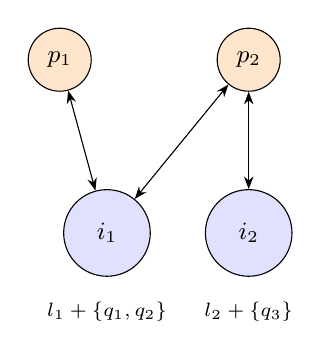
\begin{tikzpicture}[
  ent/.style={circle, draw, minimum size=8mm, font=\small, inner sep=0pt}
]
\node[ent, fill=orange!20] (p1) at (0,2.2) {$p_1$};
\node[ent, fill=orange!20] (p2) at (2.4,2.2) {$p_2$};
\node[ent, fill=blue!12, minimum size=11mm] (i1) at (0.6,0.0) {$i_1$};
\node[ent, fill=blue!12, minimum size=11mm] (i2) at (2.4,0.0) {$i_2$};
\node[font=\scriptsize, align=center] at (0.6,-1.0) {$l_1 + \{q_1,q_2\}$};
\node[font=\scriptsize, align=center] at (2.4,-1.0) {$l_2 + \{q_3\}$};
\draw[{Stealth[length=1.6mm]}-{Stealth[length=1.6mm]}] (i1) -- (p1);
\draw[{Stealth[length=1.6mm]}-{Stealth[length=1.6mm]}] (i1) -- (p2);
\draw[{Stealth[length=1.6mm]}-{Stealth[length=1.6mm]}] (i2) -- (p2);
\end{tikzpicture}
\caption{Student: paths and fused interfaces (2 stages per iteration).}
\end{subfigure}
\caption{Graph structures used by the teacher and the student, illustrated for two flows crossing two links. In the student, each interface $i$ represents a link together with all of its queues.}
\label{fig:graphs}
\end{figure}

\subsection{Fusing queues into links}

For each link $l$, the features of its queues are averaged and appended to the link's own features. Writing $\overline{(\cdot)}_l$ for the mean over $q \in \mathcal{Q}(l)$, the initial interface state is
\begin{equation}
\mathbf{h}_l^{(0)} = \mathrm{MLP}_I\Big(\big[\,\rho_l,\ \mathrm{onehot}(\pi_l),\ \overline{z(b_q)}_l,\ \overline{\mathrm{onehot}(r_q)}_l,\ \overline{w_q}_l,\ |\mathcal{Q}(l)|/3\,\big]\Big),
\label{eq:fusion}
\end{equation}
an 11-dimensional input. The averaged one-hot priority vector records which priority levels exist on the link, and the last term records how many queues it has. The fusion is computed once per forward pass with segment-mean operations and adds no trainable parameters.

\subsection{Message passing and readout}

The student uses $T = 4$ iterations of two stages and a state dimension of 16:
\begin{enumerate}
  \item \emph{Interfaces to paths:} $\mathbf{s}_p^{(k)} = \mathrm{GRU}_p\big(\mathbf{h}_{l_{p,k}},\ \mathbf{s}_p^{(k-1)}\big)$ with $\mathbf{s}_p^{(0)} = \mathbf{h}_p$, and $\mathbf{h}_p \leftarrow \mathbf{s}_p^{(|p|)}$.
  \item \emph{Paths to interfaces:} $\mathbf{h}_l \leftarrow \mathrm{GRU}_I\big(\sum_{(p,k)\,:\,l_{p,k}=l} \mathbf{s}_p^{(k-1)},\ \mathbf{h}_l\big)$.
\end{enumerate}
The path embedding uses the same 17 inputs as the teacher. The readout MLP is reduced to 16--8--8--1, and the delay is assembled exactly as in \cref{eq:readout}. The student therefore performs $4 \times 2 = 8$ message-passing stages per forward pass, one third of the teacher's 24, and has 4,505 trainable parameters (\cref{tab:params}).

\subsection{What the fusion gives up}
\label{sec:fusion-cost}

The fusion is not free of information loss, and this should be stated explicitly. In the teacher, the path GRU receives the state of the specific queue that the flow's ToS class maps to at each hop, so two flows crossing the same link in different priority classes see different queue states. In the student, every flow crossing a link sees the same interface state, and the path features (\cref{sec:teacher}) do not include the ToS class. The student therefore has no direct way to tell a high-priority flow from a low-priority flow on the same link if their traffic features are similar. Under strict-priority or weighted scheduling these flows can experience very different delays. This limitation is a deliberate trade for speed, and its likely effect on accuracy is discussed with the results in \cref{sec:discussion}.

\section{Knowledge Distillation}
\label{sec:kd}

\subsection{Distillation loss}

The student-KD model is trained with online, response-based distillation \cite{hinton2015distilling,gou2021kdsurvey}. At every training step the frozen teacher is run on the same scenario, and the student's loss combines its error against the simulator ground truth with its disagreement with the teacher:
\begin{equation}
\mathcal{L}_{\mathrm{KD}} = \alpha \cdot \underbrace{\mathrm{MAPE}\big(\mathbf{y}, \hat{\mathbf{y}}^{S}\big)}_{\text{hard loss}} \;+\; (1-\alpha) \cdot \underbrace{\frac{1}{|\mathcal{P}|}\sum_{p\in\mathcal{P}} \big(\hat{y}^{T}_p - \hat{y}^{S}_p\big)^2}_{\text{soft loss (MSE)}} ,
\label{eq:kd}
\end{equation}
where $\hat{\mathbf{y}}^{T}$ and $\hat{\mathbf{y}}^{S}$ are the teacher's and student's predictions and $\alpha = 0.5$. Only the student's parameters are updated.

Because delay is a regression target, there is no class distribution to soften with a temperature, as in the original formulation of distillation. The teacher's per-flow predictions are used directly as soft targets. They differ from the ground truth in a structured way, since they reflect what a model of this family can and cannot represent, and the hypothesis being tested is that matching them gives the student a smoother and easier target than the simulator labels alone.

\subsection{Choice of teacher}

The teacher used for distillation is the topology-diverse model (trained on 10- to 170-node topologies), not the baseline. The reason is that the student is evaluated on larger topologies than either model saw in training, and the teacher's predictions are only a useful target if they themselves extrapolate well. The results in \cref{sec:overall} confirm that the topology-diverse teacher is the more accurate of the two on the held-out set.

\section{Topology-Diverse Training Data}
\label{sec:diverse}

The dataset's original training split contains only 10-node topologies, while its original test split spans 50 to 300 nodes. To give the teacher wider coverage while still keeping a genuinely unseen test range, the data were re-split by topology size: topologies of 50 to 170 nodes were moved from the original test split into the training and validation splits, and only topologies of 200 to 300 nodes were kept for testing. Splitting by whole topology, rather than by individual scenario, ensures that no test topology was seen during training or model selection. The exact procedure and the resulting splits are given in \cref{sec:datasets}.

\section{Summary of Design Choices}

\Cref{tab:design} summarises the main design decisions and the reason for each.

\begin{table}[ht]
\centering
\small
\caption{Main design choices and their rationale.}
\label{tab:design}
\begin{tabularx}{\textwidth}{@{}p{42mm} Y@{}}
\toprule
\textbf{Choice} & \textbf{Rationale} \\
\midrule
RouteNet-Fermi as teacher & Published state-of-the-art GNN for per-flow delay with queue and scheduling support; open reference implementation and dataset. \\
Re-split by topology size & Gives the teacher wider coverage while keeping test topologies (200--300 nodes) fully unseen. \\
Merge queues into links & Removes one entity type, one GRU and two of three message-passing stages; queues are physically part of a link. \\
State dimension 16, 4 iterations & Further reduces parameters and computation; chosen as half of the teacher's settings. \\
Keep capacity-based readout & Preserves the physical structure of delay (\cref{eq:readout}), which supports extrapolation to unseen link speeds. \\
MAPE as hard loss & Relative error suits targets spanning orders of magnitude; same loss as the baseline and teacher. \\
MSE on teacher predictions & Regression target with no class distribution to soften; direct matching of predictions is the simplest response-based option. \\
\bottomrule
\end{tabularx}
\end{table}

\chapter{Experimental Setup}
\label{ch:setup}

\section{Datasets and Preprocessing}
\label{sec:datasets}

\subsection{The all-mixed dataset}

All experiments use the \emph{all-mixed} dataset published by the Barcelona Neural Networking Center together with RouteNet-Fermi \cite{ferriolgalmes2023routenetfermi,bnn2023allmixed}. Each sample is one simulated network scenario, made up of a topology, a routing and a traffic matrix, together with the per-flow mean delay measured by a packet-level simulator. Scenarios mix the four scheduling policies and several traffic models, and the topology directories carry the prefix \texttt{ch22}, indicating their origin in the 2022 edition of the Graph Neural Networking Challenge. The dataset and the reference code are distributed under the Apache License 2.0.

The dataset as downloaded is divided into three splits by topology (\cref{tab:orig-split}). The training split contains only 10-node topologies, the validation split contains five topologies of 100 to 300 nodes, and the test split contains 22 topologies of 50 to 300 nodes.

\begin{table}[ht]
\centering
\small
\caption{Original splits of the all-mixed dataset, as downloaded. Sample counts were obtained by iterating over each split with the dataset API.}
\label{tab:orig-split}
\begin{tabularx}{\textwidth}{@{}l c Y r@{}}
\toprule
\textbf{Split} & \textbf{Topologies} & \textbf{Topology sizes (nodes) and count} & \textbf{Samples} \\
\midrule
Train      & 7  & $7 \times 10$ & 11,763 \\
Validation & 5  & $1 \times$ each of 100, 150, 200, 260, 300 & 25 \\
Test       & 22 & $2 \times$ each of 50, 75, 100, 130, 170, 200, 260, 280, 300; $4 \times 240$ & 878 \\
\bottomrule
\end{tabularx}
\end{table}

A counting script that read each scenario's global (network-wide) mean delay flagged two training scenarios and one test scenario with a non-positive value. The training and evaluation pipeline does not filter scenarios, so these were not removed; for example, the evaluation of the baseline on the original test split processed all 878 scenarios.

\subsection{Topology-diverse re-split}
\label{sec:resplit}

For the teacher and both students, the data were re-split as follows. The ten topologies of 50, 75, 100, 130 and 170 nodes were moved out of the original test split. Together with the seven 10-node training topologies, they were divided so that one topology of each size (10, 50, 75, 100, 130 and 170 nodes) formed a new validation split and the remaining eleven formed a new training split. Only the twelve topologies of 200 to 300 nodes were left in the test split. The original validation split was kept aside unchanged and was not used by any of the teacher or student runs. The commands used and the resulting counts were recorded in the project log.

\begin{table}[ht]
\centering
\small
\caption{Topology-diverse splits used for the teacher and student models. Delay statistics are over the per-scenario global mean delay reported by the dataset API.}
\label{tab:v1-split}
\begin{tabularx}{\textwidth}{@{}l Y r c c@{}}
\toprule
\textbf{Split} & \textbf{Topologies (count $\times$ nodes)} & \textbf{Samples} & \textbf{Delay range} & \textbf{Mean / median} \\
\midrule
Train      & $6\times10$; $1\times$ each of 50, 75, 100, 130, 170 & 9,972 & 0.0104--2.099 & 0.217 / 0.126 \\
Validation & $1\times$ each of 10, 50, 75, 100, 130, 170          & 2,191 & 0.0103--1.874 & 0.252 / 0.135 \\
Test (OOD) & $2\times200$, $4\times240$, $2\times260$, $2\times280$, $2\times300$ & 478 & 0.0055--0.0846 & 0.0172 / 0.0106 \\
\bottomrule
\end{tabularx}
\end{table}

The counts are consistent with the original splits: the 9,972 training and 2,191 validation scenarios add up to 12,163, which equals the 11,763 original training scenarios plus the 400 scenarios contained in the ten topologies moved from the original test split ($878 - 478 = 400$).

\Cref{tab:v1-split} also shows a feature of the data that matters for interpreting the results. The mean global delay in the test split (0.0172) is more than ten times smaller than in the training split (0.217), and the two ranges barely overlap. The held-out set is therefore out of distribution in two senses: its topologies are larger than any seen in training, and its target values are concentrated at the low end of the training range. Since MAPE divides by the true delay, small absolute errors on these short delays translate into relatively large percentage errors.

\subsection{Preprocessing}

No preprocessing beyond that of the reference pipeline was applied. For each scenario, the pipeline builds the path--link--queue graph described in \cref{sec:graph} using NetworkX, computes the index tensors needed for message passing, and passes raw feature values to the model. Normalisation is done inside the models with fixed z-score statistics taken from the reference implementation; the same statistics are used by the teacher and the student. Training scenarios are shuffled by the dataset API with a fixed seed; validation and test scenarios are read in a fixed order.

\section{Implementation Details}
\label{sec:impl}

All models were implemented in Python with TensorFlow and its Keras API \cite{abadi2016tensorflow}; the project's requirements file pins TensorFlow 2.6 and NetworkX 2.6. The teacher and baseline use the RouteNet-Fermi delay model from the reference implementation without changes. The student model, the distillation training loop, the evaluation scripts and the inference benchmark were written for this project. \Cref{tab:files} lists the main files.

\begin{table}[ht]
\centering
\small
\caption{Main source files used for the reported experiments (paths relative to the project repository).}
\label{tab:files}
\begin{tabularx}{\textwidth}{@{}l Y@{}}
\toprule
\textbf{File} & \textbf{Purpose} \\
\midrule
\texttt{delay\_model.py}                   & RouteNet-Fermi delay model (baseline and teacher) \\
\texttt{student\_delay\_model.py}          & Queue-Link Fusion student model \\
\texttt{all\_mixed/data\_generator.py}     & Scenario-to-graph pipeline (reference implementation) \\
\texttt{all\_mixed/few\_shot\_all.py}      & Baseline training \\
\texttt{all\_mixed/validation\_all.py}     & Baseline evaluation \\
\texttt{all\_mixed/train\_teacher.py}      & Teacher training \\
\texttt{all\_mixed/test\_teacher.py}       & Teacher evaluation \\
\texttt{all\_mixed/student/train\_scratch.py} & Student training without distillation \\
\texttt{all\_mixed/student/train\_kd.py}   & Student training with distillation \\
\texttt{all\_mixed/student/evaluate.py}    & Student evaluation (validation and test) \\
\texttt{all\_mixed/evaluation/inference\_benchmark.py} & Latency and model-size benchmark \\
\bottomrule
\end{tabularx}
\end{table}

\paragraph{Student implementation.} The queue-to-link fusion of \cref{eq:fusion} is implemented by inverting the ragged queue-to-link index (each queue's parent link is given by the row index of the ragged tensor) and applying \texttt{tf.math.unsorted\_segment\_mean}. Unlike the reference teacher code, which constructs its recurrent layer wrappers inside the forward function, the student builds its path RNN wrapper once in the constructor, so that the compiled graph does not create new layer objects on each call.

\paragraph{Distillation implementation.} Distillation is implemented as a Keras model subclass that holds both networks and overrides the training and test steps. In each training step the teacher is called in inference mode, the student's forward pass and \cref{eq:kd} are evaluated under a gradient tape, and gradients are applied to the student's variables only. The validation step computes the student's MAPE against the ground truth. The student weights are saved whenever the validation loss improves.

\paragraph{Parameter counts.} \Cref{tab:params} breaks down the trainable parameters of both architectures. The totals agree with those reported by the benchmark script and were also checked by hand from the layer shapes (a Keras GRU cell with $d_{\mathrm{in}}$ inputs and $d$ units has $3(d_{\mathrm{in}}d + d^2 + 2d)$ parameters).

\begin{table}[ht]
\centering
\small
\caption{Trainable parameters by component.}
\label{tab:params}
\begin{tabular}{@{}l r l r@{}}
\toprule
\multicolumn{2}{c}{\textbf{Teacher (RouteNet-Fermi)}} & \multicolumn{2}{c}{\textbf{Student (Queue-Link Fusion)}} \\
\cmidrule(r){1-2}\cmidrule(l){3-4}
Path GRU (64 in, 32 units)   & 9,408 & Path GRU (16 in, 16 units)      & 1,632 \\
Link GRU (32 in, 32 units)   & 6,336 & Interface GRU (16 in, 16 units) & 1,632 \\
Queue GRU (32 in, 32 units)  & 6,336 & ---                              & --- \\
Path embedding (17--32--32)  & 1,632 & Path embedding (17--16--16)     & 560 \\
Link embedding (5--32--32)   & 1,248 & Interface embedding (11--16--16) & 464 \\
Queue embedding (5--32--32)  & 1,248 & ---                              & --- \\
Readout (32--16--16--1)      & 817   & Readout (16--8--8--1)           & 217 \\
\midrule
\textbf{Total}               & \textbf{27,025} & \textbf{Total}          & \textbf{4,505} \\
\bottomrule
\end{tabular}
\end{table}

\section{Experimental Settings}
\label{sec:settings}

\Cref{tab:settings} lists the training configuration of the four models. Settings common to all runs are: the Adam optimiser \cite{kingma2015adam} with a learning rate of $10^{-3}$; one scenario per training step (no batching across scenarios); and a global random seed of 69420 for Python, NumPy and TensorFlow, with a training-set shuffle seed of 0. Each configuration was trained once.

\begin{table}[ht]
\centering
\small
\caption{Training configuration of each model.}
\label{tab:settings}
\begin{tabularx}{\textwidth}{@{}l Y Y Y Y@{}}
\toprule
 & \textbf{Baseline} & \textbf{Teacher} & \textbf{Student-scratch} & \textbf{Student-KD} \\
\midrule
Architecture     & RouteNet-Fermi & RouteNet-Fermi & Queue-Link Fusion & Queue-Link Fusion \\
Training data    & Original train (10-node); first 10,000 shuffled scenarios & Re-split train (9,972) & Re-split train (9,972) & Re-split train (9,972) \\
Validation data  & Original validation (25) & Re-split validation (2,191) & Re-split validation (2,191) & Re-split validation (2,191) \\
Initial weights  & Reference initial-weights checkpoint & Reference initial-weights checkpoint & Random (Keras defaults) & Random (Keras defaults) \\
Loss             & MAPE & MAPE & MAPE & \cref{eq:kd}, $\alpha=0.5$ \\
Epochs $\times$ steps & $15 \times 2{,}500$ & up to $30 \times 9{,}972$ & up to $30 \times 9{,}972$ & up to $30 \times 9{,}972$ \\
Early stopping   & None & Patience 5 & Patience 5 & Patience 5 \\
Checkpoint kept  & Lowest validation MAPE & Lowest validation MAPE & Lowest validation MAPE & Lowest validation loss \\
Epochs run / best & 15 / 15 & 30 / 26 & 13 / 8 & 24 / 19 \\
Wall-clock time  & $\approx$1 h 45 min & 12 h 57 min & $\approx$5.4 h$^{\dagger}$ & $\approx$10.0 h \\
\bottomrule
\end{tabularx}

\vspace{1mm}
{\footnotesize $^{\dagger}$Taken from the project's running notes; the console log of this run was not retained (see \cref{app:logs}).}
\end{table}

\paragraph{Baseline.} The baseline follows the few-shot training script supplied with the reference implementation. It was trained twice with the same configuration. The first run kept only improving checkpoints and selected epoch 3 (validation MAPE 6.499). The second run saved every epoch and selected epoch 15 (validation MAPE 6.410). The two runs produced identical losses for the first four epochs and diverged afterwards, which is consistent with non-deterministic multi-threaded CPU kernels. The second run's checkpoint is used as \emph{the} baseline throughout this report because it is the one evaluated on the shared test set. Note that the baseline's validation split consists of 100- to 300-node topologies (\cref{tab:orig-split}), so its checkpoint was selected using larger topologies than the teacher's; this point is revisited in \cref{sec:threats}.

\paragraph{Teacher.} The teacher used the same initial weights as the baseline and ran for all 30 epochs; early stopping did not trigger because the validation loss improved at epoch 26, less than five epochs before the end.

\paragraph{Students.} Both students were initialised randomly with the same global seed. Because the distillation script builds and loads the teacher before creating the student, the random number generator is in a different state when the student's weights are drawn, so the two students do not start from identical weights. The distillation run used the teacher checkpoint from epoch 26.

\paragraph{Hardware and software.} All training and evaluation ran on a single machine running Fedora Linux, without a GPU (TensorFlow reported no CUDA device and used CPU kernels with AVX2 and FMA instructions). Training throughput was between about 147 and 178~ms per step in the runs for which console logs were kept.

\section{Evaluation Criteria and Performance Metrics}
\label{sec:metrics}

\subsection{Accuracy}

The primary accuracy metric is MAPE (\cref{eq:mape}) on the held-out test split of 478 scenarios from 200- to 300-node topologies. All four models are evaluated on exactly this set, using their selected checkpoints and without any further training or tuning. The test set was not used for checkpoint selection or for any design decision. MAPE on each model's own validation split is reported as a secondary measure.

All MAPE values reported from Keras's \texttt{evaluate} and \texttt{fit} routines are aggregated in a specific way that should be made explicit. For each scenario, Keras computes the MAPE over that scenario's flows; when averaging over scenarios, it weights each scenario by the size of the first dimension of its label tensor, which here is the number of flows. The reported value is therefore equivalent to the MAPE over all flows in the split pooled together, so larger scenarios count for more. The custom validation step in the distillation training loop, by contrast, takes an unweighted mean over scenarios. This difference is the most likely reason why the validation values recorded during distillation training differ from those obtained when the same checkpoint is evaluated afterwards (\cref{sec:kd-discrepancy}).

\subsection{Efficiency}

Efficiency is measured in four ways:
\begin{itemize}
  \item \textbf{Trainable parameters}, counted from the model variables.
  \item \textbf{Model weight size}, the parameter count multiplied by four bytes (32-bit floating point).
  \item \textbf{Message-passing stages} per forward pass (iterations times stages per iteration).
  \item \textbf{Inference latency} of a single forward pass. Each model's checkpoint is loaded, the model is called five times on one validation scenario to complete graph tracing, and then 30 further calls on the same scenario are timed with a high-resolution counter. The mean, median, standard deviation, minimum and maximum are recorded. Only the model's forward pass is timed; reading the scenario from disk and building the graph are excluded.
\end{itemize}

The benchmark was run for the baseline, the teacher and the scratch student. It was run before the distillation checkpoint existed, so student-KD was not timed separately. Student-KD has the same architecture and parameter count as student-scratch and differs only in its weight values, so its forward-pass cost is expected to be the same, but this has not been measured.

\chapter{Results and Discussion}
\label{ch:results}

This chapter reports the results of the four models described in \cref{ch:method}, evaluated as set out in \cref{ch:setup}. Every value in this chapter is taken from the saved result files and console logs listed in \cref{app:repro}. Each configuration was trained once, so differences between models are differences between single runs; this is taken into account in the discussion.

\section{Overall Experimental Results}
\label{sec:overall}

\Cref{tab:main} gives the accuracy of each model on its validation split and on the shared held-out test split of 478 scenarios from 200- to 300-node topologies. \Cref{fig:ood-bar} shows the test results graphically.

\begin{table}[ht]
\centering
\small
\caption{Accuracy of all models. Test MAPE is measured on the same 478 held-out scenarios (200--300 nodes) for every model. Validation MAPE is on each model's own validation split and is not comparable between the baseline and the other models.}
\label{tab:main}
\begin{tabular}{@{}l l c c c@{}}
\toprule
\textbf{Model} & \textbf{Architecture} & \textbf{Training topologies} & \textbf{Validation MAPE (\%)} & \textbf{Test MAPE (\%)} \\
\midrule
Baseline        & RouteNet-Fermi    & 10 nodes       & 6.41$^{a}$ & 8.40 \\
Teacher         & RouteNet-Fermi    & 10--170 nodes  & 4.71       & \textbf{5.37} \\
Student-scratch & Queue-Link Fusion & 10--170 nodes  & 10.65      & 11.92 \\
Student-KD      & Queue-Link Fusion & 10--170 nodes  & 9.04$^{b}$ & 9.83 \\
\bottomrule
\end{tabular}

\vspace{1mm}
\begin{minipage}{0.95\textwidth}
\footnotesize
$^{a}$Original validation split: 25 scenarios from five topologies of 100--300 nodes. Value recorded at the selected epoch during training.\\
$^{b}$Flow-weighted MAPE from evaluating the saved checkpoint. The unweighted value recorded during training was 9.64 (\cref{sec:kd-discrepancy}).
\end{minipage}
\end{table}

\begin{figure}[ht]
\centering
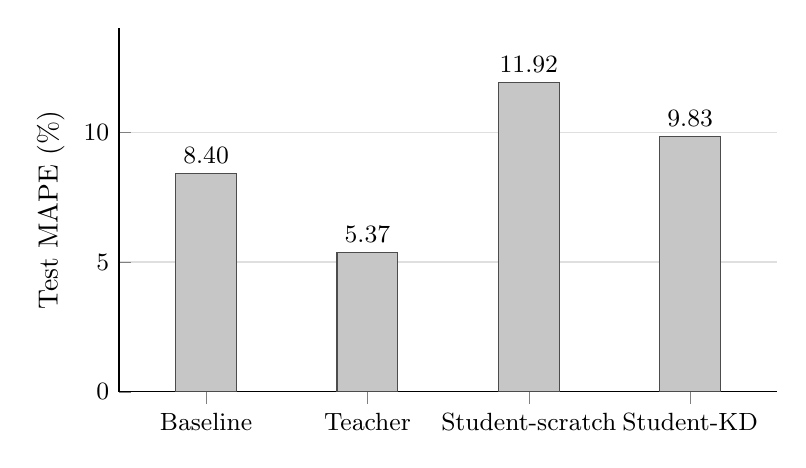
\begin{tikzpicture}
\begin{axis}[
  ybar,
  width=0.82\textwidth,
  height=6.2cm,
  bar width=22pt,
  ymin=0, ymax=14,
  ylabel={Test MAPE (\%)},
  symbolic x coords={Baseline,Teacher,Student-scratch,Student-KD},
  xtick=data,
  nodes near coords={\pgfmathprintnumber[fixed,fixed zerofill,precision=2]{\pgfplotspointmeta}},
  nodes near coords style={font=\small},
  axis lines*=left,
  ymajorgrids=true,
  grid style={gray!25},
  enlarge x limits=0.18,
  tick label style={font=\small},
]
\addplot[fill=gray!45, draw=black!70] coordinates {
  (Baseline,8.4011) (Teacher,5.3734) (Student-scratch,11.9244) (Student-KD,9.8280)
};
\end{axis}
\end{tikzpicture}
\caption{MAPE on the held-out 200--300-node test set (478 scenarios) for each model.}
\label{fig:ood-bar}
\end{figure}

Three results stand out.

\paragraph{The topology-diverse teacher is the most accurate model.} On the held-out test set the teacher's MAPE is 5.37\%, against 8.40\% for the baseline. This is a reduction of 3.03 percentage points, or 36.0\% in relative terms. The two models have identical architectures and start from the same initial weights; they differ in the training data, in the amount of training (\cref{sec:discussion}) and in the data used to select the checkpoint.

\paragraph{The compressed student loses accuracy.} Trained on the same data as the teacher but without distillation, the student reaches 11.92\% test MAPE, which is 2.22 times the teacher's error. Its validation MAPE (10.65\%) is similarly about 2.3 times the teacher's (4.71\%).

\paragraph{Distillation improves the student.} With distillation, the student's test MAPE falls from 11.92\% to 9.83\%, a reduction of 2.10 percentage points or 17.6\% in relative terms. On the validation split, MAPE falls from 10.65\% to 9.04\% (1.60 points, 15.0\%). The distilled student remains less accurate than both full-size models: its test MAPE is 4.45 points above the teacher's and 1.43 points above the baseline's.

\subsection{Training behaviour}

\Cref{fig:curves} shows the validation curves recorded during training. The teacher's validation MAPE (\cref{fig:curve-teacher}) fluctuates considerably from epoch to epoch, between 4.71\% and 6.76\% after epoch 10, even though its training loss decreases steadily. The fluctuation reflects the composition of the validation split, which holds a single topology of each size, so a change in how well the model fits one topology can move the overall value noticeably. The distillation run (\cref{fig:curve-kd}) is much smoother: its validation loss decreases almost monotonically until about epoch 15 and then levels off around 9.6--9.7\% before early stopping ends training at epoch 24. The baseline's validation curve (\cref{app:logs}) is as erratic as the teacher's, with values between 6.41\% and 8.35\% across its 15 epochs; its selected checkpoint is the last epoch, so it is possible that further training would have changed the result.

\begin{figure}[ht]
\centering
\begin{subfigure}[b]{0.49\textwidth}
\centering
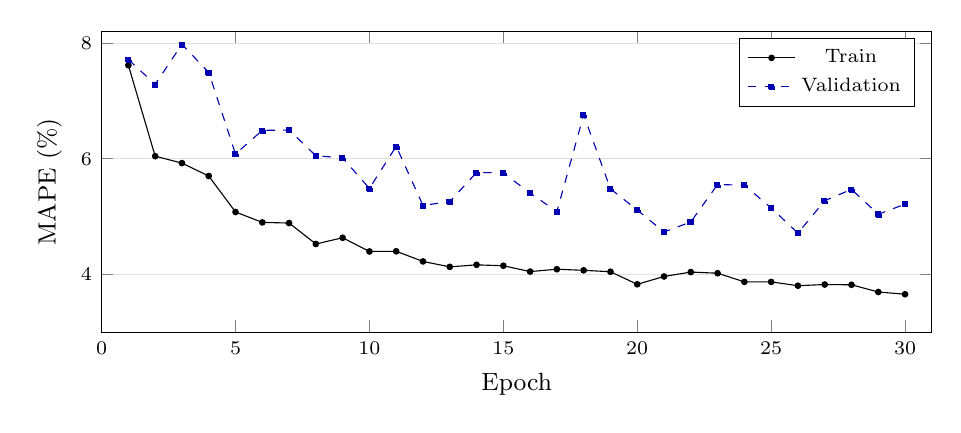
\begin{tikzpicture}
\begin{axis}[
  width=\textwidth, height=5.4cm,
  xlabel={Epoch}, ylabel={MAPE (\%)},
  xmin=0, xmax=31, ymin=3, ymax=8.2,
  legend style={font=\scriptsize, at={(0.98,0.98)}, anchor=north east},
  tick label style={font=\scriptsize}, label style={font=\small},
  ymajorgrids=true, grid style={gray!25},
]
\addplot[black, mark=*, mark size=1pt] coordinates {
(1,7.6173)(2,6.0447)(3,5.9251)(4,5.7016)(5,5.0794)(6,4.8996)(7,4.8883)(8,4.5263)(9,4.6338)(10,4.3966)
(11,4.3999)(12,4.2246)(13,4.1303)(14,4.1656)(15,4.1494)(16,4.0491)(17,4.0895)(18,4.0708)(19,4.0458)(20,3.8289)
(21,3.9641)(22,4.0405)(23,4.0208)(24,3.8710)(25,3.8707)(26,3.8044)(27,3.8249)(28,3.8205)(29,3.6957)(30,3.6569)};
\addlegendentry{Train}
\addplot[blue!70!black, dashed, mark=square*, mark size=1pt] coordinates {
(1,7.7157)(2,7.2879)(3,7.9793)(4,7.4936)(5,6.0834)(6,6.4913)(7,6.4972)(8,6.0524)(9,6.0155)(10,5.4865)
(11,6.2160)(12,5.1928)(13,5.2589)(14,5.7631)(15,5.7563)(16,5.4061)(17,5.0863)(18,6.7599)(19,5.4792)(20,5.1151)
(21,4.7331)(22,4.9076)(23,5.5545)(24,5.5437)(25,5.1506)(26,4.7139)(27,5.2744)(28,5.4711)(29,5.0402)(30,5.2150)};
\addlegendentry{Validation}
\end{axis}
\end{tikzpicture}
\caption{Teacher (best epoch 26).}
\label{fig:curve-teacher}
\end{subfigure}
\hfill
\begin{subfigure}[b]{0.49\textwidth}
\centering
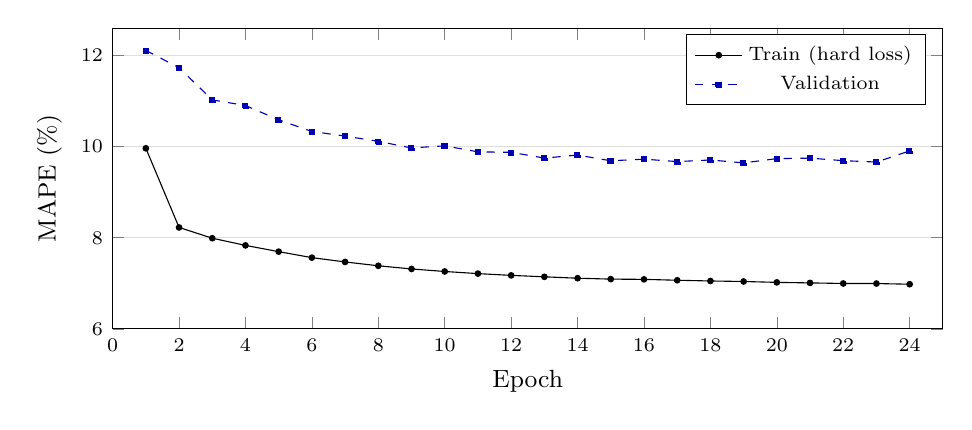
\begin{tikzpicture}
\begin{axis}[
  width=\textwidth, height=5.4cm,
  xlabel={Epoch}, ylabel={MAPE (\%)},
  xmin=0, xmax=25, ymin=6, ymax=12.6,
  legend style={font=\scriptsize, at={(0.98,0.98)}, anchor=north east},
  tick label style={font=\scriptsize}, label style={font=\small},
  ymajorgrids=true, grid style={gray!25},
]
\addplot[black, mark=*, mark size=1pt] coordinates {
(1,9.9645)(2,8.2266)(3,7.9904)(4,7.8328)(5,7.6954)(6,7.5641)(7,7.4693)(8,7.3852)(9,7.3156)(10,7.2600)
(11,7.2133)(12,7.1745)(13,7.1431)(14,7.1124)(15,7.0925)(16,7.0871)(17,7.0677)(18,7.0516)(19,7.0404)(20,7.0209)
(21,7.0095)(22,6.9965)(23,6.9952)(24,6.9804)};
\addlegendentry{Train (hard loss)}
\addplot[blue!70!black, dashed, mark=square*, mark size=1pt] coordinates {
(1,12.1137)(2,11.7319)(3,11.0272)(4,10.9029)(5,10.5883)(6,10.3335)(7,10.2322)(8,10.1161)(9,9.9722)(10,10.0181)
(11,9.8867)(12,9.8760)(13,9.7496)(14,9.8157)(15,9.6898)(16,9.7258)(17,9.6723)(18,9.7076)(19,9.6439)(20,9.7374)
(21,9.7480)(22,9.6928)(23,9.6622)(24,9.9065)};
\addlegendentry{Validation}
\end{axis}
\end{tikzpicture}
\caption{Student-KD (best epoch 19).}
\label{fig:curve-kd}
\end{subfigure}
\caption{Per-epoch MAPE recorded during training. For the student-KD run, both curves are unweighted means over scenarios (\cref{sec:metrics}), and the training curve shows only the hard (ground-truth) term of the loss.}
\label{fig:curves}
\end{figure}

\section{Comparison with Existing Methods}
\label{sec:comparison}

The existing method against which this work is compared is RouteNet-Fermi itself, represented by the baseline (trained according to the reference implementation's few-shot script on the original 10-node training data) and by the teacher (the same architecture trained on topology-diverse data). Published RouteNet-Fermi figures are not quoted for comparison because they were obtained with a different training budget and evaluation protocol, and the aim here is a like-for-like comparison on one test set.

For completeness, \cref{tab:hist} also records the baseline's results on the dataset's original test split, which spans 50 to 300 nodes and therefore includes topologies that were later moved into the teacher's training data. These numbers are not comparable with the teacher and student results, but they show that the baseline's error on the 200- to 300-node subset (8.40\%) is similar to its error on the full original test set (8.22\%) with the same checkpoint. The first training run, selected at epoch 3, gave a higher error of 9.17\% on the original test split, which illustrates how much a single run and the choice of checkpoint can move the result.

\begin{table}[ht]
\centering
\small
\caption{Baseline results on the two test sets. Only the last row is comparable with the teacher and student results in \cref{tab:main}.}
\label{tab:hist}
\begin{tabular}{@{}l l c c@{}}
\toprule
\textbf{Run (checkpoint)} & \textbf{Test set} & \textbf{Scenarios} & \textbf{MAPE (\%)} \\
\midrule
Run 1 (epoch 3)  & Original test, 50--300 nodes   & 878 & 9.17 \\
Run 2 (epoch 15) & Original test, 50--300 nodes   & 878 & 8.22 \\
Run 2 (epoch 15) & Held-out test, 200--300 nodes  & 478 & 8.40 \\
\bottomrule
\end{tabular}
\end{table}

Other classes of method discussed in \cref{ch:related}, such as queueing-theory models, packet simulation and graph-free distilled students, were not run in this project, so no quantitative comparison with them is claimed.

\section{Additional Analyses}
\label{sec:analyses}

\subsection{Model size and inference latency}
\label{sec:efficiency}

\Cref{tab:efficiency} reports the efficiency measurements. The student has 83.3\% fewer trainable parameters than RouteNet-Fermi (4,505 against 27,025, a ratio of 6.0), its weights occupy 17.6~KB against 105.6~KB, and it performs one third of the message-passing stages. A single forward pass on the benchmark scenario took 34.2~ms on average for the student, against 178.5~ms for the teacher and 177.5~ms for the baseline, making the student about 5.2 times faster. The student's latency was also much more stable, with a standard deviation of 1.8~ms against 9.4--13.0~ms for the full-size models. The baseline and teacher, which share an architecture, have the same latency within measurement noise, as expected.

\begin{table}[ht]
\centering
\small
\caption{Model size and single-forward-pass latency on CPU (30 timed runs after 5 warm-up runs, one validation scenario). Student-KD shares the student architecture and was not timed separately.}
\label{tab:efficiency}
\begin{tabular}{@{}l r r c c c c c@{}}
\toprule
\multirow{2}{*}{\textbf{Model}} & \multirow{2}{*}{\textbf{Params}} & \multirow{2}{*}{\textbf{Size (KB)}} & \multirow{2}{*}{\textbf{MP stages}} & \multicolumn{3}{c}{\textbf{Latency (ms)}} & \multirow{2}{*}{\textbf{Speed-up}} \\
\cmidrule(lr){5-7}
 & & & & Mean & Median & Std & \\
\midrule
Baseline        & 27,025 & 105.6 & 24 & 177.5 & 175.5 & 13.0 & 1.01$\times$ \\
Teacher         & 27,025 & 105.6 & 24 & 178.5 & 177.6 & 9.4  & 1.00$\times$ \\
Student-scratch & 4,505  & 17.6  & 8  & 34.2  & 33.9  & 1.8  & 5.22$\times$ \\
Student-KD      & 4,505  & 17.6  & 8  & \multicolumn{3}{c}{not measured} & --- \\
\bottomrule
\end{tabular}
\end{table}

\Cref{fig:tradeoff} places the four models on a plane of test error against model size. No model is better than the others on both axes. The teacher gives the lowest error at full size; the distilled student gives the lowest error among the small models.

\begin{figure}[ht]
\centering
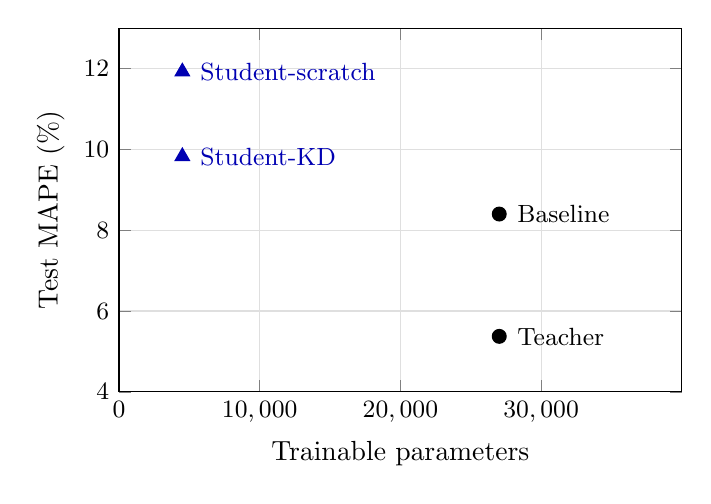
\begin{tikzpicture}
\begin{axis}[
  width=0.72\textwidth, height=6.2cm,
  xlabel={Trainable parameters}, ylabel={Test MAPE (\%)},
  xmin=0, xmax=40000, ymin=4, ymax=13,
  xtick={0,10000,20000,30000},
  clip=false,
  scaled x ticks=false,
  xticklabel style={/pgf/number format/.cd, fixed, 1000 sep={,}},
  ymajorgrids=true, xmajorgrids=true, grid style={gray!25},
  tick label style={font=\small},
  nodes near coords, point meta=explicit symbolic,
  nodes near coords style={font=\small, anchor=west, xshift=3pt},
]
\addplot[only marks, mark=*, mark size=2.5pt] coordinates {
  (27025,8.4011) [Baseline]
  (27025,5.3734) [Teacher]
};
\addplot[only marks, mark=triangle*, mark size=3pt, blue!70!black] coordinates {
  (4505,11.9244) [Student-scratch]
  (4505,9.8280) [Student-KD]
};
\end{axis}
\end{tikzpicture}
\caption{Test MAPE against number of trainable parameters. Circles: RouteNet-Fermi; triangles: Queue-Link Fusion.}
\label{fig:tradeoff}
\end{figure}

\subsection{End-to-end evaluation time}

The forward-pass benchmark excludes reading the scenario and building its graph. The evaluation logs give a complementary view of total processing time on the large test topologies. Evaluating the 478 test scenarios took 9,307~s for the baseline, 9,642~s for the teacher, 8,938~s for student-scratch and 9,032~s for student-KD, which is roughly 19--20~s per scenario for every model. Since a fivefold difference in forward-pass cost changed the total by only about 7\%, most of the per-scenario time in this pipeline is spent outside the model. The pipeline was not profiled, but the likely candidates are parsing the simulator output and building the graph with NetworkX in Python. The student's speed advantage is therefore real for the model itself, but a deployment would also need a faster graph-construction step to benefit from it fully.

\subsection{Generalisation gap}

For the three models trained on the topology-diverse split, the difference between test and validation MAPE indicates how much accuracy is lost when moving from topologies of up to 170 nodes to topologies of 200 to 300 nodes. The gap is 0.66 points for the teacher (4.71\% to 5.37\%), 1.28 points for student-scratch (10.65\% to 11.92\%) and 0.78 points for student-KD (9.04\% to 9.83\%). The distilled student's gap is closer to the teacher's than to that of the student trained from scratch. This is consistent with the student having absorbed some of the teacher's behaviour on larger topologies, although with a single run per model the difference between 0.78 and 1.28 points cannot be treated as established.

\subsection{Validation metric discrepancy in the distillation run}
\label{sec:kd-discrepancy}

The distillation training run recorded a best validation MAPE of 9.64\% at epoch 19, but evaluating the saved epoch-19 checkpoint afterwards gave 9.04\% on the same validation split. The saved checkpoint is the one written at epoch 19 (the evaluation log loads \texttt{ckpt-19}), so the difference is not due to loading the wrong weights. The likely cause is the aggregation difference described in \cref{sec:metrics}. The custom validation step in the distillation loop averages per-scenario MAPE with equal weight per scenario, while Keras's \texttt{evaluate} weights each scenario by its number of flows. Larger topologies contain many more flows, so a lower flow-weighted value means that the student is more accurate, in relative terms, on the larger validation topologies than on the smaller ones. This explanation follows from the code; it has not been confirmed by recomputing both aggregates from saved per-scenario predictions.

Two consequences follow. First, the 9.04\% figure is the one comparable with all other validation values in this report, which were obtained through the same Keras routines. Second, the distillation run selected its checkpoint with a slightly different criterion from the other runs. With the per-scenario curve flat between epochs 15 and 23 (\cref{fig:curve-kd}), a flow-weighted criterion might have selected a different epoch, but the difference is unlikely to be large.

\subsection{Relative size of the distillation loss terms}

At the selected epoch of the distillation run, the mean training values of the two terms in \cref{eq:kd} were 7.04 for the hard MAPE term and 0.169 for the soft MSE term, giving a total of $0.5 \times 7.04 + 0.5 \times 0.169 = 3.60$, which matches the logged total of 3.6045. The soft term therefore made up only about 2.3\% of the loss value. This does not mean that the teacher signal had a negligible effect, because what matters for training is the gradient of each term and Adam rescales update magnitudes, but it does mean that $\alpha = 0.5$ should not be read as an even split of influence between the ground truth and the teacher. The MSE is computed on raw delay values, which are small for most flows and large for a few, so the soft term is likely to be dominated by the flows with the longest delays.

\section{Discussion of Findings}
\label{sec:discussion}

\subsection{Topology diversity and the full-size models}

The clearest result is that the teacher, trained on topologies of up to 170 nodes, is substantially more accurate on 200- to 300-node topologies than the baseline trained only on 10-node topologies. Learning delay behaviour on larger networks, with longer paths and more flows sharing each link, appears to transfer better to even larger networks than learning it on very small ones. This finding is relevant beyond this project: when preparing training data for a learned network model, including topologies closer in size to the target deployment is likely to help more than additional samples from small topologies.

The comparison is not perfectly controlled, however. The teacher was trained for about 299,000 steps ($30 \times 9{,}972$), while the baseline followed the reference few-shot script with 37,500 steps ($15 \times 2{,}500$), about one eighth as many. The baseline's best checkpoint was its last, so it may not have converged. Part of the teacher's advantage could therefore come from longer training rather than from the more diverse data. A baseline trained on 10-node data for the same number of steps would separate the two effects.

\subsection{The cost of compression}

The scratch student's error is 2.2 times the teacher's, so the compression in its current form has a significant accuracy cost. Several features of the design may contribute, and the results do not identify which matters most.
\begin{itemize}
  \item \textbf{Loss of per-queue information.} As explained in \cref{sec:fusion-cost}, a flow in the student sees the average state of all queues on a link, not the state of the queue it actually uses, and the flow features do not include its ToS class. Under strict-priority and weighted scheduling, flows of different classes on the same link can have very different delays, and the student has no direct way to distinguish them.
  \item \textbf{Fewer message-passing iterations.} With four iterations instead of eight, information travels a shorter distance through the graph before the readout. On 200- to 300-node topologies, where paths are long and many flows interact, this may limit how well the student captures congestion caused by distant traffic.
  \item \textbf{Smaller hidden states.} Halving the state dimension reduces the capacity of every component, including the readout that estimates occupancy.
  \item \textbf{Shorter training.} The scratch student stopped after 13 epochs with its best result at epoch 8, whereas the teacher continued to improve until epoch 26. With a noisy validation signal and a patience of five epochs, early stopping may have ended training before the student converged.
\end{itemize}
An ablation that changes these factors one at a time, for example a student that keeps separate queue states but uses four iterations, would show which of them accounts for most of the gap.

\subsection{The effect of distillation}

Distillation reduced the student's test MAPE by 2.10 points and its validation MAPE by 1.60 points, and the distilled student's generalisation gap was closer to the teacher's. These are consistent improvements on two independent splits, and they support the hypothesis that the teacher's predictions provide a useful training signal for a structurally different student.

Three caveats limit how strongly this can be stated. First, there is one run of each configuration, and the two students started from different random weights because of the way the distillation script initialises the teacher first (\cref{sec:settings}). Without repeated runs, the variation between seeds is unknown and could in principle be comparable to the observed difference. Second, the distillation run trained for longer before stopping (best epoch 19 against 8), so part of the gain may come from a training trajectory that happened to avoid early stopping, rather than from the teacher's predictions as such. Third, as shown above, the soft term is numerically small and dominated by long-delay flows, so the mechanism by which it helps is not clear from these experiments.

Even with these caveats, distillation did not close the gap to the full-size models. The distilled student remains 4.45 points behind the teacher and 1.43 points behind the baseline on the test set. Under the conditions tested, a student of this size trained on diverse topologies with distillation is less accurate than a full RouteNet-Fermi trained on small topologies only.

\subsection{Practical trade-off}

The results describe a trade-off rather than a single best model. If accuracy on large, unseen networks is the priority, the topology-diverse RouteNet-Fermi teacher is clearly preferable, at about 178~ms per forward pass on the test machine. If the model must be evaluated many times, for example to rank many candidate routings on a constrained controller, the distilled student offers roughly five times more forward passes for the same compute at a test MAPE of about 9.8\%. Whether that error is acceptable depends on the use. For ranking candidate configurations, what matters is whether the model orders them correctly, which a model with a moderate absolute error may still do well. This was not measured here (\cref{sec:future}).

\subsection{Threats to validity}
\label{sec:threats}

The following limitations should be kept in mind when interpreting the results.
\begin{itemize}
  \item \textbf{Single runs.} Every configuration was trained once. Run-to-run variation is unknown. The baseline's two runs, which diverged after four epochs and selected different checkpoints, gave 9.17\% and 8.22\% on the original test set, which suggests the variation can be substantial.
  \item \textbf{Confounds between baseline and teacher.} Besides training data, the two differ in the number of training steps and in the validation data used for checkpoint selection. The baseline's validation split contains 100- to 300-node topologies, which is closer in size to the test set than the teacher's validation split; if anything, this favours the baseline.
  \item \textbf{Aggregate metric only.} Results are reported as a single flow-weighted MAPE over the test set. Errors were not broken down by topology size, scheduling policy or traffic model, so it is not known where each model's errors concentrate.
  \item \textbf{Shift in the target distribution.} Test delays are about an order of magnitude smaller than training delays (\cref{tab:v1-split}), and MAPE is sensitive to errors on small targets. Absolute error metrics were not computed.
  \item \textbf{Latency measurement.} Latency was measured on one scenario from the validation split, on one CPU-only machine, for the forward pass only. The size of that scenario was not recorded, and the distilled student was not timed separately.
  \item \textbf{Lost log.} The console log of the scratch student's training run was overwritten. Its per-epoch values come from the project notes, although the saved checkpoint files are consistent with them (\cref{app:logs}). Its evaluation results come from a separate evaluation log, which was kept.
  \item \textbf{Simulated data and scope.} All data come from a packet-level simulator. No experiment was run on an SDN controller or with real traffic, and only delay was modelled.
\end{itemize}

\chapter{Conclusion}
\label{ch:conclusion}

\section{Summary of Research and Key Findings}

This project asked whether a lightweight GNN, distilled from a topology-diverse RouteNet-Fermi teacher, can predict per-flow delay at a much lower cost, and how much accuracy it loses on networks larger than those used in training.

\textbf{Objective 1.} RouteNet-Fermi trained on 10- to 170-node topologies reached 5.37\% MAPE on held-out 200- to 300-node topologies, against 8.40\% when trained on 10-node topologies only, a 36\% relative reduction. Part of this gain may come from the teacher's longer training.

\textbf{Objective 2.} The Queue-Link Fusion student merges each link with its queues, reducing the graph to two entity types, the message passing from 24 to 8 stages, and the parameters from 27,025 to 4,505, while keeping the capacity-based delay readout. Its forward pass was 4.4 to 7.9 times faster on a CPU, with the gain growing with network size. End to end, however, it saved only about 8\%, because building the input graph took about 90\% of the time.

\textbf{Objective 3.} The student reached 11.92\% test MAPE from scratch, about twice the teacher's error. A first distillation run lowered this to 9.83\%, but that comparison was not controlled. In a controlled re-test with three paired seeds, identical initial weights and a relative soft loss, distillation was better in two pairs and worse in one, on both validation and test (mean test difference $+0.50$ points), and showed no consistent benefit. The student's training error already exceeded the teacher's validation error, so its limit is capacity rather than guidance. In a six-switch Mininet/Ryu emulation, the frozen teacher and both students ranked three candidate paths in the measured order of mean delay, chose a path with 8.8\% lower delay than the hop-count default, and predicted the measured delays within about 5--7\%; the students scored the candidates about twice as fast as the teacher. This shows that the models can work as route scorers in a controller, but not that they choose better than simple rules, since a least-loaded rule would have made the same choice. Physical checks block impossible predictions before any route is installed.

Overall, diverse training topologies improved accuracy on larger networks, but compressing the model cost more accuracy than that diversity gained: the small model on diverse data remained less accurate than the full-size model on 10-node data. Under controlled conditions, distillation did not recover that accuracy. The compressed model cut the model's own cost by 4 to 8 times, but in this pipeline building the input graph, not the model, dominated the end-to-end cost.

\section{Research Contributions}

\begin{enumerate}
  \item An out-of-distribution evaluation of RouteNet-Fermi using a documented topology-level re-split of the all-mixed dataset, with errors broken down by topology size.
  \item The Queue-Link Fusion student, a bipartite GNN for per-flow delay prediction with 83\% fewer parameters and one third of the message-passing stages, with its information loss stated explicitly and its accuracy--speed trade-off measured across network sizes.
  \item A controlled, paired study of response-based distillation for a network-modelling regression task, showing no consistent benefit and explaining why: the student is limited by capacity, and the reference training setup is noisy.
  \item An end-to-end cost analysis showing that input-graph construction, not the model, dominates the cost of one prediction in this pipeline.
  \item A controlled Mininet/Ryu integration in which frozen GNN models score candidate routes, with physical prediction checks that block impossible predictions.
  \item A check of the reference converter's hop ordering, measured as negligible both offline and in the emulation.
\end{enumerate}

\section{Future Work}
\label{sec:future}

\begin{itemize}
  \item Pass each flow's ToS class into the student's path update to recover per-class queue information.
  \item Reduce training noise with scenario-level shuffling, a decaying learning rate and a per-topology validation average, then repeat the paired distillation study with more seeds.
  \item Try richer distillation: match the teacher's per-hop queue occupancies, or train the student on extra scenarios labelled by the teacher.
  \item Build the input graph once per network and update it incrementally, so that the student's speed-up reaches the end-to-end cost when many configurations are evaluated.
  \item Train the 10-node baseline with the same budget as the teacher to separate the effects of data and training length.
  \item Break offline errors down by scheduling policy and traffic model.
  \item Repeat the emulation under several pre-declared traffic loads, topologies and packet phase offsets, compare the models with simple rules such as least-loaded routing, and measure total decision-to-install time.
  \item Adapt the models to real traffic with labelled real-traffic data, as the RouteNet-Fermi authors did, and extend them to jitter and loss.
  \item Apply pruning and quantisation, alone and with distillation.
\end{itemize}


% ---------------------------------------------------------------------
\bibliographystyle{IEEEtran}
\bibliography{references}

% ---------------------------------------------------------------------
\appendix
\chapter{Reproducibility}
\label{app:repro}

The code is in the project repository. The all-mixed dataset \cite{bnn2023allmixed} is expected under \path{data/}: the original splits in \path{data/all_mixed/} (used by the baseline) and the re-split in \path{data/all_mixed_v1/} (used by the teacher and students). The re-split validation set contains the topologies \path{topo-10-7}, \path{topo-50-0}, \path{topo-75-10}, \path{topo-100-20}, \path{topo-130-26} and \path{topo-170-34}.

\begin{table}[H]
\centering
\footnotesize
\caption{Main scripts, selected checkpoints and result files.}
\label{tab:repro}
\begin{tabularx}{\textwidth}{@{}p{22mm} Y >{\raggedright\arraybackslash}p{66mm}@{}}
\toprule
\textbf{Step} & \textbf{Script (directory)} & \textbf{Checkpoint / output} \\
\midrule
Baseline        & \path{few_shot_all.py}, \path{validation_all.py} (\path{all_mixed/}) & \path{ckpt_dir_0_10000/15-6.41}, \path{results_baseline_ood.json} \\
Teacher         & \path{train_teacher.py}, \path{test_teacher.py} (\path{all_mixed/}) & \path{ckpt_dir_0_9972/ckpt-26}, \path{results_teacher.json} \\
Student-scratch & \path{train_scratch.py} (\path{all_mixed/student/}) & \path{ckpt_dirs_scratch/ckpt-08} \\
Student-KD      & \path{train_kd.py} (\path{all_mixed/student/}) & \path{ckpt_dirs_kd_alpha0.5/ckpt-19} \\
Student tests   & \path{evaluate.py} (\path{all_mixed/student/}) & \path{results_student.json} \\
Latency         & \path{inference_benchmark.py} (\path{all_mixed/evaluation/}) & \path{inference_benchmark_results.json} \\
Emulation       & \path{run.py} (\path{mininet_experiment/}) & \path{outputs/six_validation_summary.json} \\
\bottomrule
\end{tabularx}
\end{table}

The emulation is run from the repository root. For example, a model-driven run and a forced-path measurement are started with:
{\footnotesize
\begin{verbatim}
sudo python mininet_experiment/run.py --method kd \
     --seconds 60 --name kd_60_01
sudo python mininet_experiment/run.py --method shortest \
     --candidate 1 --seconds 60 --name path1_new
\end{verbatim}
}
\noindent A model's predictions can be checked without Mininet by running \path{model_worker.py} with the model name and the \path{--check} option.

\paragraph{Notes on the files.}
\begin{itemize}
  \item As committed, \path{validation_all.py} evaluates the original test split and writes \path{results_all.json} (8.22\%). The held-out result in \path{results_baseline_ood.json} (8.40\%) was produced by running the same script with \path{TEST_PATH} set to \path{data/all_mixed_v1/test} and the output file renamed; the console output of that run is in \path{all_mixed/baseline_ood.log}.
  \item The emulation's raw outputs (\path{mininet_experiment/outputs/}, including \path{six_validation_summary.json}, \path{six_validation_predictions.json} and \path{author_real_traffic/}) are excluded from the Git repository. They are kept with the research data backups, and their contents are summarised in \path{mininet_experiment/README.md}.
  \item The console log of the scratch student's training run was not kept; only its checkpoints and evaluation log remain.
\end{itemize}


\end{document}
